\documentclass[a4paper,12pt]{article}
\usepackage{graphicx, float, enumerate, parskip}
%\usepackage[indonesian]{babel}
\usepackage{amsmath, amsthm, amssymb, amsfonts}
\theoremstyle{definition}
\newtheorem{definition}{Definisi}[section]
\newtheorem{theorem}{Teorema}[section]
\newtheorem{example}{Contoh}[section]
\usepackage{listings, fancyvrb, spverbatim, xcolor}
\lstset{% setup listings
    language=R,% set programming language
    frame=tb,
    basicstyle=\ttfamily\small,% basic font style
    keywordstyle=\color{blue},% keyword style
    commentstyle=\color{gray},% comment style
    breaklines=true,% automatic line breaking
    fancyvrb=true,% verbatim code is typset by listings
}
\usepackage[
    backend=biber,
    style=bwl-FU,
    sorting=nyt,
    maxbibnames=99,
    natbib=true,
]
{biblatex}
\addbibresource{DPustaka.bib}


%% ---------------------------
\begin{document}
    \title{Template Paper Pemodelan Statistika dan Simulasi}
    \author{
    Nama Mahasiswa 4112320035 \\
    Nama Mahasiswa 4112320036
    }
\date{\today}
\begin{titlepage}
    \maketitle
\end{titlepage}

\tableofcontents

\newpage
\section{Pendahuluan}
Model pembelajaran mesin didefinisikan menggunakan parameter tertentu untuk menghasilkan program komputer dengan mengoptimalkan parameter model menggunakan data pelatihan atau pengalaman masa lalu. Pembelajaran mesin menggunakan analisis statistik untuk menghasilkan model, karena tujuan utamanya adalah membuat kesimpulan dari sampel pelatihan. Dalam beberapa kasus, efisiensi algoritme pelatihan mungkin sama pentingnya dengan keakuratan klasifikasinya. Teknik pembelajaran mesin digunakan di berbagai bidang sebagai sistem pendukung keputusan \citep{Alpaydın2020}.


\section{Apa itu Machine Learning}
Menurut \cite{Kulkarni2012} dijelaskan bahwa pembelajaran mesin adalah studi tentang algoritme komputer untuk membantu merumuskan prediksi dan reaksi yang akurat dalam keadaan tertentu, atau untuk bertindak secara cerdas. Secara umum, pembelajaran mesin adalah tentang belajar untuk menciptakan keadaan yang lebih baik di masa depan berdasarkan apa yang telah dipelajari di masa lalu. Mesin belajar dari informasi, pengetahuan, dan pengalaman yang ada; karenanya, pembelajaran mesin adalah pengembangan program yang memungkinkan kita menganalisis data dari berbagai sumber dengan memilih data yang relevan dan memanfaatkan data tersebut untuk memprediksi perilaku sistem dalam skenario yang serupa atau berbeda. Pembelajaran mesin juga mengklasifikasikan objek dan aktivitas untuk mendukung keputusan skenario input baru. Motivasi pembelajaran mesin adalah bahwa kecerdasan dan pembelajaran tambahan diperlukan untuk mengatasi situasi yang tidak pasti.




\subsection{Memahami Machine Learning}
Pembelajaran mesin menjadi populer pada 1990-an ketika para peneliti mulai menjadikannya subbidang kecerdasan buatan (AI) yang menonjol karena algoritme yang meminjam ide dari probabilitas, statistik, dan AI lebih berhasil daripada model tetap berbasis aturan yang memerlukan upaya manual. Selain itu, pembelajaran mesin adalah bidang multidisiplin yang terus berkembang dari waktu ke waktu dan terus berkembang. Jelas, itu berkembang dengan cepat sejak 1990-an dengan penemuan mesin vektor pendukung, hutan acak, jaringan memori jangka pendek panjang (LSTM), dan kemajuan kerangka kerja di mesin dan pembelajaran mendalam yang mencakup scikit-learn, PyTorch, TensorFlow, dan Theano. Munculnya sistem cerdas, termasuk IBM Watson, DeepFace, dan AlphaGo, dimulai baru-baru ini \citep{Sarkar2018}.







\section{Pengantar Belajar Latex} 
\subsection{Cara menuliskan Equation}
Misalkan $X_1,X_2,...,X_n$ adalah sampel random dari distribusi dengan parameter $\theta$ yang tidak diketahui. Statistik $Y=u(X_1,X_2,...,X_n)$ disebut dengan statistik cukup untuk $\theta$, jika distribusi bersyarat dari $X_1,X_2,...,X_n$ diberikan $Y$ tidak bergantung pada parameter $\theta$

\begin{equation*}
    f_{X|s}(x_1,x_2,...,x_n)=
    \begin{cases}
    f(x_1, x_2, ..., x_n;\theta), & \text{jika} ~ sigma(x_1,x_2,...,x_n)=s \\ 
    0, & \text{yang lainnya}.
    \end{cases}
\end{equation*}


\subsection{Cara membuat Listing dan Output}
Berikut contoh membuat listing 
\begin{lstlisting}
contoh listing

\end{lstlisting}


Berikut contoh membuat output kode dengan verbatim 
\begin{spverbatim}
contoh output verbatim
    
\end{spverbatim}


\subsection{Cara input Gambar dan Tabel}
Berikut ini cara menginput Gambar
\begin{figure}[H]
    \centering
    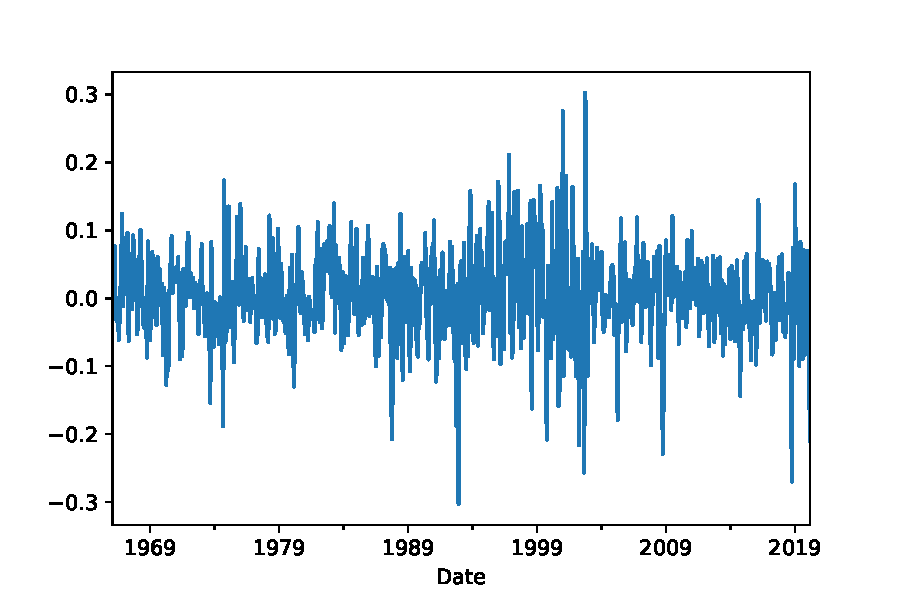
\includegraphics[width=0.8\textwidth]{gb/Gam9-6-IBMDiff.pdf}
    \caption{Plot runtun waktu harga penutupan dari saham IBM}
    \label{Gam9-6-IBMDiff}
\end{figure}

Berikut ini adalah contoh membuat Tabel.
\begin{table}[H]
    \centering
    \begin{tabular}{lccc}
    \hline
    & MA($q$) & AR($p$) & ARMA($p,q$) $(p>0, q>0)$ \\
    \hline
    ACF & xxx & xxx  & xxx \\
    PACF  & xxx & xxx $p$ & xxx \\
    \hline
    \end{tabular}
    \caption{Perilaku ACF dan PACF model ARMA}
    \label{Tab-3.01-ACFPACF}
\end{table}


\subsection{Cara menulis Definisi, Teorema, dan Contoh}
Berikut contoh membuat Definisi
\begin{definition}[Variabel Random] % Opsi menambahkan keterangan

Contoh Definisi
\end{definition}


Berikut contoh membuat Contoh
\begin{example}[Aplikasi ...]

Contoh Definisi
\end{example}


Berikut contoh membuat Teorema
\begin{theorem}[Teorema Limit Pusat] 

Contoh Definisi
\end{theorem}


\newpage
\printbibliography[heading=bibintoc,title={Daftar Pustaka}]
\end{document}